\chapter{Diagrammes binaires solide--liquide}\label{ch:b2:solid-liquid-diagrams}

L'étain fond à \qty{232}{\degreeCelsius} et le plomb à \qty{327}{\degreeCelsius},
et pourtant l'ancienne soudure des électriciens, un mélange des deux, fond à
\qty{182}{\degreeCelsius}, au-dessous de l'un et de l'autre. Le sel répandu sur une route fait fondre la glace, mais seulement
jusque vers \qty{-21}{\degreeCelsius}~; par une nuit plus froide, il ne sert à rien.
Le cuivre et le nickel, en revanche, se mélangent en toutes proportions même à l'état
solide, et leurs alliages fondent sur un intervalle de températures compris entre celles des
deux métaux. Les diagrammes de ce chapitre indiquent, pour chaque couple, quels solides
cristallisent d'un liquide qui refroidit, à quelles températures et en quelles
quantités --- le savoir qui sous-tend chaque coulée, chaque soudure et chaque
alliage à bas point de fusion.

\begin{recall}
\Cref{ch:b2:chemical-potential}~: \omterm{def:b2:chemical-potential:chemical-potential}{potentiel chimique} d'un constituant dans un \omterm{def:b2:chemical-potential:ideal-mixture}{mélange
idéal}, cryométrie. \Cref{ch:b2:equilibrium-shifts}~: la \omterm{def:b2:equilibrium-shifts:variance}{variance}.
\Cref{ch:b2:liquid-vapour-diagrams}~: \omterm{def:b2:liquid-vapour-diagrams:binary-diagram}{diagrammes binaires}, conodales et \omterm{thm:b2:liquid-vapour-diagrams:lever}{règle
des moments}. Le volume de première année~: liaison métallique, alliages de substitution et
d'insertion, types de cristaux.
\end{recall}

\begin{omfigure}
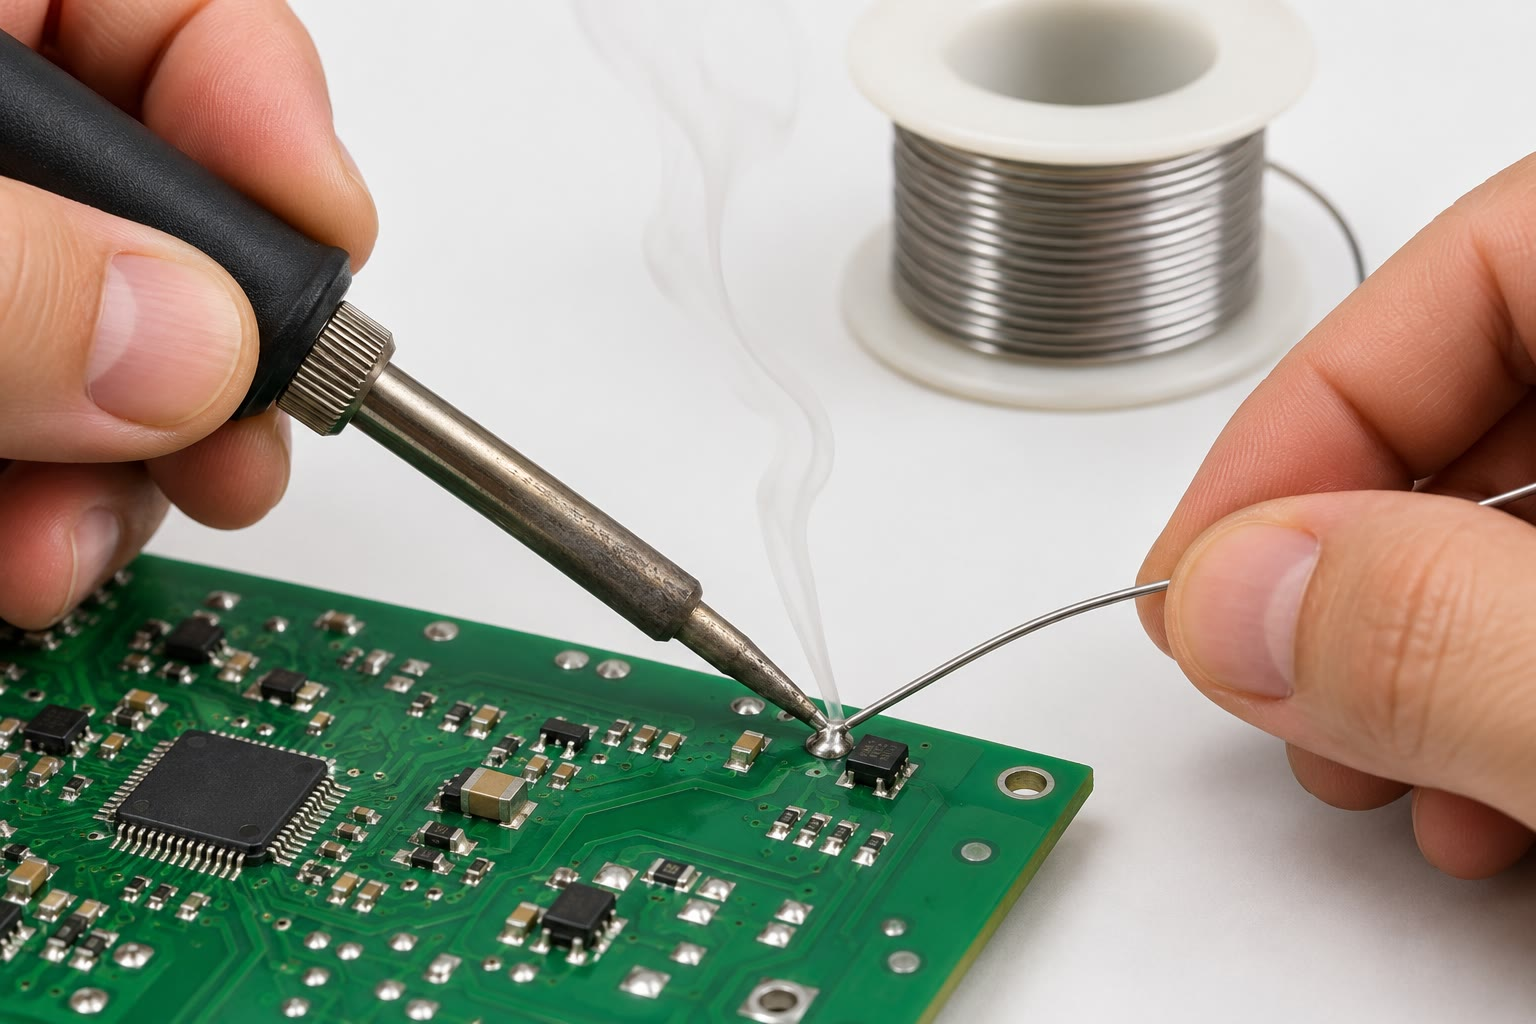
\includegraphics[width=0.6\linewidth]{images/book3/ai/b2-08-soldering.jpg}

{\small Soudure d'un composant sur une carte électronique~: le fil de soudure fond au
contact du fer chaud et le joint se fige en moins d'une seconde quand on retire le fer
--- parce que l'alliage fond à une température unique et basse.}
\end{omfigure}

\section{L'analyse thermique}

\begin{definition}[Analyse thermique]\label{def:b2:solid-liquid-diagrams:cooling-curve}
L'\emph{analyse thermique}\index{analyse thermique} détermine les températures
des changements d'état d'un échantillon à partir de sa température enregistrée pendant qu'on le
chauffe ou qu'on le refroidit à vitesse régulière. L'enregistrement de la température en fonction du temps
au cours d'un refroidissement lent est une \emph{courbe de refroidissement}\index{courbe de refroidissement}.
\end{definition}

Loin de tout changement d'état, l'échantillon se refroidit régulièrement. Quand un solide commence à
cristalliser, la chaleur de cristallisation ralentit le refroidissement~: la courbe présente une
rupture de pente, ou s'arrête un moment à température constante --- un
\textit{palier} --- si la solidification a lieu à température fixée.

\begin{proposition}[Paliers]\label{prop:b2:solid-liquid-diagrams:plateaus}
À pression fixée, un corps pur se solidifie à température constante, de même
qu'un liquide binaire d'où cristallisent ensemble deux solides. Un liquide binaire
d'où cristallise un seul solide se solidifie sur un intervalle de températures.
\end{proposition}

\begin{proof}
La pression étant fixée, la \omterm{def:b2:equilibrium-shifts:variance}{variance} est $v = n - r + 1 - \varphi$. Corps
pur, liquide + solide~: $v = 1 + 1 - 2 = 0$. Binaire, liquide + deux solides~:
$v = 2 + 1 - 3 = 0$. Binaire, liquide + un solide~: $v = 2 + 1 - 2 = 1$~: la
température varie en même temps que la composition du liquide. Une \omterm{def:b2:equilibrium-shifts:variance}{variance} nulle signifie que la
température ne peut pas varier tant que toutes les phases sont présentes~: la chaleur évacuée est
fournie par la solidification, jusqu'à la disparition d'une phase.
\end{proof}

\begin{omfigure}
\begin{tikzpicture}[font=\small, x=0.55cm, y=0.05cm]
  \foreach \dx/\name in {0/métal pur, 9/{mélange, un solide d'abord}, 18/mélange eutectique} {
    \draw[->] (\dx,0) -- (\dx+7.5,0) node[below left, font=\scriptsize] {$t$};
    \draw[->] (\dx,0) -- (\dx,62) node[above, font=\scriptsize] {$T$};
    \node[font=\scriptsize] at (\dx+3.8,-8) {\name};
  }
  % pure: cool, plateau at 40, cool
  \draw[omDef, thick] (0,58) .. controls (1,48) and (1.6,42) .. (2,40) -- (4.5,40) .. controls (5.2,32) and (6,24) .. (7,20);
  \node[font=\scriptsize, anchor=south] at (3.25,40.5) {palier};
  % mixture: cool, break at 48, slow fall, plateau at 30, cool
  \draw[omDef, thick] (9,58) .. controls (9.6,53) and (9.9,50) .. (10.2,48)
     .. controls (11,42) and (11.6,35) .. (12.3,30) -- (14.2,30) .. controls (14.9,23) and (15.6,17) .. (16.5,14);
  \node[font=\scriptsize, anchor=west] at (10.4,49.5) {rupture};
  \node[font=\scriptsize, anchor=south] at (13.25,30.5) {eutectique};
  % eutectic: plateau at 30
  \draw[omDef, thick] (18,58) .. controls (19,46) and (19.8,36) .. (20.5,30) -- (24,30) .. controls (24.7,23) and (25.4,17) .. (26.2,14);
  \node[font=\scriptsize, anchor=south] at (22.25,30.5) {palier};
\end{tikzpicture}

{\small \omterm{def:b2:solid-liquid-diagrams:cooling-curve}{Courbes de refroidissement}, schéma. Un métal pur se solidifie sur un palier. Un
mélange présente une rupture de pente quand le premier solide apparaît, puis le refroidissement
lent d'un liquide qui se solidifie sur un intervalle de températures, puis le
palier de l'eutectique. Un liquide de composition eutectique se solidifie sur un
palier unique, comme un corps pur.}
\end{omfigure}

\begin{method}[Construire un diagramme à partir de courbes de refroidissement]\label{met:b2:solid-liquid-diagrams:diagram-from-curves}
\begin{enumerate}
  \item Enregistrer les \omterm{def:b2:solid-liquid-diagrams:cooling-curve}{courbes de refroidissement} d'une série de compositions, constituants purs
        compris.
  \item Sur un graphique (composition, température), placer pour chaque composition la
        température de la première rupture (le début de la cristallisation) et de
        chaque palier.
  \item Joindre les points de début de cristallisation~: c'est le \omterm{def:b2:solid-liquid-diagrams:liquidus}{liquidus}. Joindre
        les fins de solidification~: le \omterm{def:b2:solid-liquid-diagrams:liquidus}{solidus}. Un palier observé à la même
        température pour de nombreuses compositions est une ligne invariante (un eutectique).
  \item La longueur du palier eutectique, maximale pour la composition
        eutectique, permet de situer cette composition.
\end{enumerate}
\end{method}

\section{Miscibilité totale à l'état solide}

\begin{definition}[Solution solide]\label{def:b2:solid-liquid-diagrams:solid-solution}
Une \emph{solution solide}\index{solution solide} est une phase cristalline unique de
composition variable, dans laquelle des atomes d'un constituant remplacent des atomes de
l'autre sur les sites d'un même réseau (substitution) ou occupent les sites interstitiels de
ce réseau (insertion).
\end{definition}

Le cuivre et le nickel ont la même structure cubique à faces centrées et des atomes de
rayons voisins~: ils forment une \omterm{def:b2:solid-liquid-diagrams:solid-solution}{solution solide} de substitution en toute composition.

\begin{definition}[Liquidus et solidus]\label{def:b2:solid-liquid-diagrams:liquidus}
Sur un diagramme solide--liquide, le \emph{liquidus}\index{liquidus} est la courbe
au-dessus de laquelle tout est liquide~; il donne la composition du liquide en
équilibre avec un solide. Le \emph{solidus}\index{solidus} est la courbe au-dessous
de laquelle tout est solide~; lorsque le solide est une solution, il donne la
composition du solide en équilibre avec le liquide.
\end{definition}

\begin{proposition}[Le fuseau]\label{prop:b2:solid-liquid-diagrams:lens}
Si les deux constituants forment des solutions idéales à l'état liquide et à l'état solide,
le \omterm{def:b2:solid-liquid-diagrams:liquidus}{liquidus} et le \omterm{def:b2:solid-liquid-diagrams:liquidus}{solidus} joignent les deux températures de fusion et délimitent un
domaine diphasé en forme de fuseau~; à chaque température, les fractions molaires $x_i$ de
chaque constituant dans le liquide et dans le solide sont liées par
\[
  \frac{x_i^{\ell}}{x_i^{s}} = \exp\left[-\frac{\Delta_{\text{fus}}H_i}{R}\left(\frac1T - \frac1{T_i^*}\right)\right] .
\]
\end{proposition}

\begin{proof}
Le \omterm{def:b2:chemical-potential:chemical-potential}{potentiel chimique} de $i$ est le même dans les deux phases, $\mu_i^{*,s} +
RT\ln x_i^s = \mu_i^{*,\ell} + RT\ln x_i^\ell$, donc $RT\ln(x_i^\ell/x_i^s) =
-(\mu_i^{*,\ell} - \mu_i^{*,s}) = -\Delta_{\text{fus}}G_i(T)$, et avec
$\Delta_{\text{fus}}H_i$ constante, $\Delta_{\text{fus}}G_i = \Delta_{\text{fus}}H_i(1 - T/T_i^*)$.
Avec $x_1 + x_2 = 1$ dans chaque phase, les deux relations fixent les deux
compositions à chaque $T$ (résolution numérique pour la figure)~; on admet que
les courbes obtenues forment un fuseau.
\end{proof}

\begin{omfigure}
\begin{tikzpicture}
\begin{axis}[omphase, width=0.62\linewidth, height=7cm, ymin=1050, ymax=1480,
  xlabel={$x$ (nickel)}, ylabel={$T$ (\unit{\degreeCelsius})}]
\addplot[omliquidus] table[x=xl, y=T] {figdata/out/bachelor-2-solid-liquid-a.dat};
\addplot[omsolidus] table[x=xs, y=T] {figdata/out/bachelor-2-solid-liquid-a.dat};
\draw[tieline] (axis cs:0.541,1300) -- (axis cs:0.609,1300);
\fill (axis cs:0.58,1300) circle (1.3pt);
\node[font=\scriptsize] at (axis cs:0.25,1400) {liquide};
\node[font=\scriptsize] at (axis cs:0.8,1150) {solution solide};
\node[font=\scriptsize, anchor=east] at (axis cs:0.5,1330) {liquidus};
\node[font=\scriptsize, anchor=west] at (axis cs:0.66,1290) {solidus};
\node[font=\scriptsize, anchor=west] at (axis cs:0.03,1080) {\qty{1085}{\degreeCelsius}};
\draw[black!50] (axis cs:0.005,1084) -- (axis cs:0.03,1080);
\node[font=\scriptsize, anchor=south east] at (axis cs:1.0,1456) {\qty{1455}{\degreeCelsius}};
\end{axis}
\end{tikzpicture}

{\small Cuivre--nickel, calculé pour des \omterm{def:b2:solid-liquid-diagrams:solid-solution}{solutions solide} et liquide idéales à partir des
températures et des enthalpies de fusion des deux métaux. À
\qty{1300}{\degreeCelsius}, un alliage de composition 0.58 se partage en un liquide
de 0.541 et un solide de 0.609 (conodale en tirets).}
% ledger: tfus:Cu, dfus:Cu, tfus:Ni, dfus:Ni
\end{omfigure}

\begin{method}[Lire un diagramme solide--liquide]\label{met:b2:solid-liquid-diagrams:read-solid-liquid}
\begin{enumerate}
  \item Suivre vers le bas la verticale de la composition globale à partir du
        liquide.
  \item Sur le \omterm{def:b2:solid-liquid-diagrams:liquidus}{liquidus}, le premier solide apparaît~; sa composition se lit à
        l'autre extrémité de la conodale (le \omterm{def:b2:solid-liquid-diagrams:liquidus}{solidus}, ou un constituant pur).
  \item Dans le domaine diphasé, lire les deux compositions aux extrémités de la
        conodale et les proportions par la \omterm{thm:b2:liquid-vapour-diagrams:lever}{règle des moments}, en moles avec les fractions
        molaires, en masse avec les fractions massiques.
  \item Sur une ligne invariante horizontale, la température s'arrête jusqu'à la disparition
        d'une phase~; au-dessous, lire le nouveau couple de phases.
\end{enumerate}
\end{method}

\begin{example}[Un alliage à \qty{1300}{\degreeCelsius}]\label{ex:b2:solid-liquid-diagrams:lever}
Pour l'alliage de fraction molaire en nickel 0.58 à \qty{1300}{\degreeCelsius}, la
fraction des atomes présents dans le solide vaut $(0.58 - 0.541)/(0.609 - 0.541) = 0.57$.
Le premier solide qui apparaît, vers \qty{1315}{\degreeCelsius}, est plus riche en nickel
que l'alliage, le dernier liquide plus pauvre.
\end{example}

Le diagramme décrit l'équilibre, qui dans un solide s'établit lentement~: les premiers cristaux,
riches en nickel, se recouvrent de couches de plus en plus pauvres en nickel à mesure que le liquide
évolue, et la diffusion dans le solide n'a pas le temps de les uniformiser. Une pièce coulée
refroidie rapidement est formée de cristaux \textit{zonés}, dont la composition varie du cœur au
bord~; un long chauffage au-dessous du \omterm{def:b2:solid-liquid-diagrams:liquidus}{solidus} les homogénéise.

\section{Miscibilité nulle à l'état solide~: l'eutectique}

Lorsque les deux solides ne se mélangent pas du tout, chaque constituant cristallise pur, et
le \omterm{def:b2:solid-liquid-diagrams:liquidus}{liquidus} comporte deux branches, une par solide.

\begin{theorem}[Schröder--van Laar]\label{thm:b2:solid-liquid-diagrams:schroder}
Si un constituant A cristallise pur à partir d'un mélange liquide idéal, la branche du \omterm{def:b2:solid-liquid-diagrams:liquidus}{liquidus}
sur laquelle apparaît le solide A est donnée par
\[
  \ln x_A = -\frac{\Delta_{\text{fus}}H_A}{R}\Big(\frac1T - \frac1{T_A^*}\Big),
\]
où $x_A$ est la fraction molaire de A dans le liquide, $T_A^*$ et
$\Delta_{\text{fus}}H_A$ la température et l'enthalpie de fusion de A pur
(supposée constante).
\end{theorem}

\begin{proof}
À l'équilibre, le \omterm{def:b2:chemical-potential:chemical-potential}{potentiel chimique} de A solide pur est égal à celui de A dans le
liquide~: $\mu_A^{*,s}(T) = \mu_A^{*,\ell}(T) + RT\ln x_A$. D'où $R\ln x_A =
-\Delta_{\text{fus}}G_A(T)/T$. D'après Gibbs--Helmholtz, $d(\Delta_{\text{fus}}G_A/T)/
dT = -\Delta_{\text{fus}}H_A/T^2$~; l'intégration de $T_A^*$, où
$\Delta_{\text{fus}}G_A = 0$, à $T$ donne $\Delta_{\text{fus}}G_A/T =
\Delta_{\text{fus}}H_A(1/T - 1/T_A^*)$.
\end{proof}

Pour une solution diluée, $\ln x_A = \ln(1 - x_B) \approx -x_B$ et $1/T -
1/T_A^* \approx -\Delta T/T_A^{*2}$~: $\Delta T = RT_A^{*2}x_B/\Delta_{\text{fus}}H_A$,
la loi de la cryométrie du \cref{ch:b2:chemical-potential}. Pour le benzène ($T^* =
\qty{278.64}{K}$, $\Delta_{\text{fus}}H = \qty{9.87}{kJ/mol}$, $M =
\qty{78.11}{g/mol}$), la \omterm{def:b2:chemical-potential:colligative}{constante cryoscopique} $RT^{*2}M/\Delta_{\text{fus}}H$
vaut \qty{5.11}{K.kg/mol}.
% ledger: tfus:benzene, dfus:benzene

\begin{definition}[Eutectique]\label{def:b2:solid-liquid-diagrams:eutectic}
Le \emph{point eutectique}\index{point eutectique} d'un système binaire est le
point où le liquide est en équilibre avec deux solides à la fois~; c'est la
plus basse température à laquelle un liquide existe dans cette partie du diagramme. Un
liquide de composition eutectique, et le mélange fin et intime des deux
solides dans lequel il se solidifie, sont appelés un \emph{mélange
eutectique}\index{melange eutectique@mélange eutectique}.
\end{definition}

\begin{corollary}[L'eutectique est à la rencontre des branches du liquidus]\label{cor:b2:solid-liquid-diagrams:eutectic}
Pour deux constituants non miscibles à l'état solide et idéaux à l'état liquide, la
température eutectique $T_E$ et la composition eutectique sont solutions de
$x_A(T_E) + x_B(T_E) = 1$, chaque $x$ étant donné par la relation de Schröder--van Laar
de son propre solide.
\end{corollary}

\begin{proof}
À l'eutectique, le liquide est saturé en les deux solides~: il se trouve sur les deux
branches à la fois, avec la même composition lue en A et en B.
\end{proof}

\begin{omfigure}
\begin{tikzpicture}
\begin{axis}[omphase, width=0.62\linewidth, height=6.5cm, ymin=-25, ymax=85,
  xlabel={$x$ (naphtalène)}, ylabel={$T$ (\unit{\degreeCelsius})}]
\addplot[omliquidus] table[x=x, y=T] {figdata/out/bachelor-2-solid-liquid-b-benzene.dat};
\addplot[omliquidus] table[x=x, y=T] {figdata/out/bachelor-2-solid-liquid-b-naphthalene.dat};
\draw[thick] (axis cs:0,-3.55) -- (axis cs:1,-3.55);
\fill (axis cs:0.133,-3.55) circle (1.5pt);
\node[font=\scriptsize, anchor=north] at (axis cs:0.133,-4.5) {E};
\node[font=\scriptsize] at (axis cs:0.45,72) {liquide};
\node[font=\scriptsize, align=center] at (axis cs:0.65,22) {liquide + naphtalène\\ solide};
\node[font=\scriptsize, anchor=south west] at (axis cs:0.08,45) {liquide + benzène solide};
\draw[thin] (axis cs:0.12,45) -- (axis cs:0.06,0.8);
\node[font=\scriptsize] at (axis cs:0.55,-15) {benzène solide + naphtalène solide};
\end{axis}
\end{tikzpicture}

{\small Benzène--naphtalène, calculé avec la relation de Schröder--van Laar
pour chaque solide. Les deux branches se rejoignent à l'eutectique E,
\qty{-3.5}{\degreeCelsius} et 0.13 de naphtalène, au-dessous duquel tout est solide.}
% ledger: tfus:benzene, dfus:benzene, tfus:naphthalene, dfus:naphthalene
\end{omfigure}

\begin{example}[Refroidissement d'un mélange benzène--naphtalène]\label{ex:b2:solid-liquid-diagrams:naphthalene}
Un liquide de fraction molaire en naphtalène 0.5 se refroidit jusqu'à la branche du naphtalène
sur le \omterm{def:b2:solid-liquid-diagrams:liquidus}{liquidus}, vers \qty{46}{\degreeCelsius}, où du naphtalène solide pur
commence à cristalliser. Le liquide, qui perd du naphtalène, descend le long de la
branche~; à \qty{-3.5}{\degreeCelsius}, il atteint l'eutectique, et le reste
se solidifie à température constante en \omterm{def:b2:solid-liquid-diagrams:eutectic}{mélange eutectique}. D'après la \omterm{thm:b2:liquid-vapour-diagrams:lever}{règle des moments},
juste au-dessus de l'eutectique, le naphtalène solide représente $(0.5 - 0.133)/(1 - 0.133) =
42~\%$ des moles, le liquide eutectique 58~\%.
\end{example}

\begin{proposition}[Longueur du palier eutectique]\label{prop:b2:solid-liquid-diagrams:plateau-length}
Pour des échantillons de même masse refroidis avec la même puissance évacuée, la
durée du palier eutectique est proportionnelle à la quantité de liquide qui
atteint l'eutectique, maximale pour la composition eutectique et nulle pour les
constituants purs.
\end{proposition}

\begin{proof}
Sur le palier, la température est constante~: la chaleur évacuée, $\Phi\,\Delta t$
avec une puissance constante $\Phi$, est la chaleur libérée par la solidification du
liquide eutectique, $m_E\,\Delta_{\text{fus}}h_E$. Donc $\Delta t = m_E\,\Delta_{\text{fus}}h_E/
\Phi$, proportionnelle à la masse $m_E$ de liquide eutectique, que donne la \omterm{thm:b2:liquid-vapour-diagrams:lever}{règle
des moments}.
\end{proof}

\section{Miscibilité partielle et composés définis}

La plupart des couples de métaux ne sont ni totalement miscibles ni totalement non miscibles à l'état
solide~: chacun dissout un peu de l'autre. Le plomb dissout jusqu'à 19~\% d'étain
en masse, l'étain jusqu'à 3.4~\% de plomb. Le diagramme comporte alors deux \omterm{def:b2:solid-liquid-diagrams:solid-solution}{solutions
solides}, (Pb) et (Sn), et un eutectique entre elles~; la ligne eutectique
n'atteint plus les bords du diagramme, mais s'arrête aux limites des \omterm{def:b2:solid-liquid-diagrams:solid-solution}{solutions
solides}.

\begin{omfigure}
\begin{tikzpicture}[font=\small, x=0.075cm, y=0.022cm]
  \draw[->] (0,0) -- (106,0) node[right] {\% Sn (masse)};
  \draw[->] (0,0) -- (0,360) node[above] {$T$ (\unit{\degreeCelsius})};
  \foreach \t in {100,200,300} \draw (0,\t) -- (-1.5,\t) node[left, font=\scriptsize] {\t};
  \foreach \w in {0,20,40,60,80,100} \draw (\w,0) -- (\w,-5) node[below, font=\scriptsize] {\w};
  % invariant points (NIST): Pb 327.5, Sn 231.9, eutectic 182.2 at 62.13; limits 18.91 and 96.59
  \draw[omliquidus] (0,327.5) .. controls (25,290) and (45,235) .. (62.13,182.2);
  \draw[omliquidus] (100,231.9) .. controls (85,215) and (72,200) .. (62.13,182.2);
  \draw[omsolidus] (0,327.5) .. controls (8,280) and (14,220) .. (18.91,182.2);
  \draw[omsolidus] (100,231.9) .. controls (98.5,215) and (97.5,200) .. (96.59,182.2);
  \draw[thick] (18.91,182.2) -- (96.59,182.2);
  \draw[omsolidus, densely dashed] (18.91,182.2) .. controls (12,120) and (6,60) .. (3,20);
  \draw[omsolidus, densely dashed] (96.59,182.2) .. controls (98.5,120) and (99.3,60) .. (99.6,20);
  \fill (62.13,182.2) circle (1.5pt);
  \fill (18.91,182.2) circle (1.2pt); \fill (96.59,182.2) circle (1.2pt);
  \node[anchor=south, font=\scriptsize] at (62.13,186) {E};
  \node[font=\scriptsize] at (55,300) {liquide};
  \node[font=\scriptsize] at (6,150) {(Pb)};
  \node[font=\scriptsize] at (103,140) {(Sn)};
  \node[font=\scriptsize] at (28,235) {L + (Pb)};
  \node[font=\scriptsize] at (84,192) {L + (Sn)};
  \node[font=\scriptsize] at (55,100) {(Pb) + (Sn)};
  % cooling path at 40 %
  \draw[->, omProp, thick] (40,340) -- (40,30);
  \node[font=\scriptsize, omProp, anchor=south] at (40,342) {40~\%};
  \node[font=\scriptsize, anchor=north east] at (16.6,179) {18.9};
  \node[font=\scriptsize, anchor=north] at (62.13,178) {62.1};
  \node[font=\scriptsize, anchor=north east] at (95.8,178) {96.6};
  \node[font=\scriptsize, anchor=west] at (101,182.2) {\qty{182.2}{\degreeCelsius}};
\end{tikzpicture}

{\small Le diagramme plomb--étain, tracé à partir de ses points invariants~: températures de
fusion du plomb (\qty{327.5}{\degreeCelsius}) et de l'étain (\qty{231.9}{\degreeCelsius}),
eutectique E à \qty{182.2}{\degreeCelsius} et 62.1~\% d'étain, limites des \omterm{def:b2:solid-liquid-diagrams:solid-solution}{solutions
solides} à la température eutectique (18.9~\% et 96.6~\% d'étain). Les courbes
entre ces points, et les limites de solubilité en tirets au-dessous de l'eutectique,
sont tracées de façon schématique. Flèche~: le refroidissement d'une soudure à 40~\%.}
% ledger: eut:Pb-Sn.T, eut:Pb-Sn.wL, eut:Pb-Sn.wPb, eut:Pb-Sn.wSn, tfus:Pb, tfus:Sn
\end{omfigure}

Une soudure à 40~\% d'étain commence à se solidifier sur le \omterm{def:b2:solid-liquid-diagrams:liquidus}{liquidus} en déposant des cristaux de
la solution riche en plomb (Pb)~; le liquide s'enrichit en étain jusqu'à ce que, à
\qty{182.2}{\degreeCelsius}, il atteigne la composition eutectique et se solidifie en
un mélange fin de lamelles de (Pb) et de (Sn), autour des cristaux primaires.

\begin{omfigure}
\begin{tikzpicture}[font=\small]
  \begin{scope}
    \clip (0,0) circle (2.2);
    \fill[gray!20] (-2.3,-2.3) rectangle (2.3,2.3);
    \foreach \k in {-24,...,24} \draw[gray!65, line width=1.1pt] (-2.4+0.2*\k,-2.4) -- ++(55:6);
    \foreach \cx/\cy/\r/\a in {-0.9/0.8/0.55/10, 0.7/1.0/0.45/40, 0.2/-0.6/0.6/-20, -1.1/-0.9/0.4/70, 1.3/-0.3/0.35/5} {
      \fill[omDef!35, draw=omDef, rotate around={\a:(\cx,\cy)}] (\cx,\cy) ellipse ({\r} and {0.7*\r});
    }
  \end{scope}
  \draw[thick] (0,0) circle (2.2);
  \draw[<-, omProp, thick] (0.7,1.0) -- (3.0,1.6) node[right, text=black] {cristal primaire de (Pb)};
  \draw[<-, omProp, thick] (1.6,0.9) -- (3.0,0.5) node[right, text=black, align=left] {eutectique~: lamelles\\ alternées de (Pb) et de (Sn)};
\end{tikzpicture}

{\small La microstructure d'une soudure à 40~\% d'étain après un refroidissement lent, schéma~:
des cristaux primaires de (Pb), formés entre le \omterm{def:b2:solid-liquid-diagrams:liquidus}{liquidus} et l'eutectique, dans une
matrice d'eutectique faite de fines plaquettes alternées des deux \omterm{def:b2:solid-liquid-diagrams:solid-solution}{solutions
solides}.}
\end{omfigure}

\begin{definition}[Composé défini]\label{def:b2:solid-liquid-diagrams:defined-compound}
Un \emph{composé défini}\index{compose defini@composé défini} est un solide de
composition fixée $\mathrm{A}_a\mathrm{B}_b$ formé par les deux constituants. Il présente
une \emph{fusion congruente}\index{fusion congruente} lorsqu'il fond en donnant un liquide de
sa propre composition~: le \omterm{def:b2:solid-liquid-diagrams:liquidus}{liquidus} présente alors un maximum à cette composition.
\end{definition}

Un composé à \omterm{def:b2:solid-liquid-diagrams:defined-compound}{fusion congruente} partage le diagramme en deux~: chaque moitié, A avec
$\mathrm{A}_a\mathrm{B}_b$ et $\mathrm{A}_a\mathrm{B}_b$ avec B, est un diagramme à
part entière, avec son propre eutectique. La composition du maximum, lue en fraction
molaire, donne la formule du composé.

\begin{omfigure}
\begin{tikzpicture}[font=\small, x=6cm, y=0.05cm]
  \draw[->] (0,0) -- (1.06,0) node[right] {$x_{\mathrm B}$};
  \draw[->] (0,0) -- (0,95) node[above] {$T$};
  \node[below, font=\scriptsize] at (0,0) {A}; \node[below, font=\scriptsize] at (1,0) {B};
  \node[below, font=\scriptsize] at (0.667,0) {$\tfrac23$};
  \draw[omliquidus] (0,70) .. controls (0.12,58) and (0.25,45) .. (0.35,35);
  \draw[omliquidus] (0.35,35) .. controls (0.45,62) and (0.58,79) .. (0.667,80);
  \draw[omliquidus] (0.667,80) .. controls (0.75,79) and (0.8,68) .. (0.85,50);
  \draw[omliquidus] (0.85,50) .. controls (0.9,56) and (0.95,62) .. (1,65);
  \draw[thick] (0,35) -- (0.667,35); \draw[thick] (0.667,50) -- (1,50);
  \draw[thick] (0.667,0) -- (0.667,80);
  \fill (0.35,35) circle[radius=1.5pt]; \fill (0.85,50) circle[radius=1.5pt];
  \fill (0.667,80) circle[radius=1.5pt];
  \node[anchor=north, font=\scriptsize] at (0.35,34) {E$_1$};
  \node[anchor=north, font=\scriptsize] at (0.85,49) {E$_2$};
  \node[anchor=south, font=\scriptsize] at (0.667,81) {fusion de $\mathrm{AB_2}$};
  \node[font=\scriptsize] at (0.35,80) {liquide};
  \node[font=\scriptsize, align=center] at (0.33,15) {A +\\ $\mathrm{AB_2}$};
  \node[font=\scriptsize, align=center] at (0.84,25) {$\mathrm{AB_2}$\\ + B};
\end{tikzpicture}

{\small Diagramme schématique comportant un \omterm{def:b2:solid-liquid-diagrams:defined-compound}{composé défini} $\mathrm{AB_2}$ (droite
verticale en $x_{\mathrm B} = 2/3$) à \omterm{def:b2:solid-liquid-diagrams:defined-compound}{fusion congruente} au maximum du
\omterm{def:b2:solid-liquid-diagrams:liquidus}{liquidus}. Le diagramme est formé de deux diagrammes à eutectique simple accolés, d'eutectiques
E$_1$ et E$_2$.}
\end{omfigure}

\section{Applications}

\paragraph{Soudures et alliages à bas point de fusion.} Une soudure doit fondre au-dessous des pièces
qu'elle assemble et se figer vite, sans domaine pâteux~: la composition eutectique est
le choix naturel. L'eutectique étain--plomb fond à \qty{182.2}{\degreeCelsius}~;
le plomb étant toxique, l'électronique utilise aujourd'hui des soudures sans plomb, parmi lesquelles
l'eutectique bismuth--étain, qui fond à \qty{138.8}{\degreeCelsius} et contient
57~\% de bismuth en masse.
% ledger: eut:Pb-Sn.T, eut:Bi-Sn.T, eut:Bi-Sn.wL

\paragraph{Déneigement.} La glace et le sel forment un eutectique~: l'eutectique glace--chlorure de sodium
dihydraté se situe à \qty{252}{K} (\qty{-21}{\degreeCelsius}) et 23.3~\% de chlorure
de sodium en masse. Au-dessus de cette température, le sel au contact de la glace forme une
saumure dont la température de congélation est inférieure à celle de la route, et la glace
fond~; au-dessous, aucun liquide ne peut exister, et le sel est inutile.
% ledger: eut:NaCl-water.T, eut:NaCl-water.w

\paragraph{Cristallisation.} Le diagramme d'un sel et de l'eau se lit comme tout
autre~: refroidir une solution chaude saturée fait franchir la courbe de solubilité (le
\omterm{def:b2:solid-liquid-diagrams:liquidus}{liquidus} du sel), et des cristaux purs du sel se déposent tandis que les
impuretés, trop diluées pour atteindre leur propre \omterm{def:b2:solid-liquid-diagrams:liquidus}{liquidus}, restent dans les eaux mères.
C'est la purification par recristallisation du volume de première année, lue sur un
diagramme.

\begin{omfigure}
\begin{tikzpicture}
\begin{axis}[omphase, width=0.62\linewidth, height=6cm, xmin=0, xmax=100,
  ymin=90, ymax=285, xlabel={\% Bi (masse)}, ylabel={$T$ (\unit{\degreeCelsius})}]
\addplot[omliquidus] table[x=w, y=T] {figdata/out/bachelor-2-solid-liquid-d-Sn.dat};
\addplot[omliquidus] table[x=w, y=T] {figdata/out/bachelor-2-solid-liquid-d-Bi.dat};
\draw[densely dashed] (axis cs:0,119.5) -- (axis cs:100,119.5);
\fill[omThm] (axis cs:56.97,138.8) circle (2pt);
\node[font=\scriptsize, omThm, anchor=west] at (axis cs:64,129) {eutectique évalué};
\draw[omThm, thin] (axis cs:64,129) -- (axis cs:57.8,137.6);
\node[font=\scriptsize, anchor=north] at (axis cs:52,118) {modèle idéal};
\node[font=\scriptsize] at (axis cs:50,250) {liquide};
\end{axis}
\end{tikzpicture}

{\small Bismuth--étain~: les branches du \omterm{def:b2:solid-liquid-diagrams:liquidus}{liquidus} prévues pour des solides purs et un liquide
idéal (Schröder--van Laar, en bleu) se rejoignent à un eutectique vers
\qty{120}{\degreeCelsius}~; l'eutectique évalué (point rouge) se situe à
\qty{138.8}{\degreeCelsius} et 57~\% de bismuth.}
% ledger: tfus:Sn, dfus:Sn, tfus:Bi, dfus:Bi, eut:Bi-Sn.T, eut:Bi-Sn.wL
\end{omfigure}

\section{Exercices}

\begin{exercise}[$\star$]\label{exo:b2:solid-liquid-diagrams:1}
Sur le diagramme cuivre--nickel, donner les phases présentes à
\qty{1300}{\degreeCelsius} pour des fractions molaires en nickel de 0.40, 0.58 et 0.70.
\end{exercise}

\begin{exercise}[$\star$]\label{exo:b2:solid-liquid-diagrams:2}
\qty{2.00}{mol} d'un alliage cuivre--nickel de fraction molaire en nickel 0.58 sont maintenues
à \qty{1300}{\degreeCelsius}. Calculer les quantités de solide et de liquide, ainsi que la
quantité de nickel dans chacun.
\end{exercise}

\begin{exercise}[$\star$]\label{exo:b2:solid-liquid-diagrams:3}
Calculer la \omterm{def:b2:equilibrium-shifts:variance}{variance} à pression fixée (a) d'un métal pur pendant sa solidification~;
(b) d'un alliage cuivre--nickel pendant sa solidification~; (c) d'un liquide plomb--étain sur la
ligne eutectique.
\end{exercise}

\begin{exercise}[$\star$]\label{exo:b2:solid-liquid-diagrams:4}
Tracer l'allure de la \omterm{def:b2:solid-liquid-diagrams:cooling-curve}{courbe de refroidissement} de l'étain pur de \qty{300}{\degreeCelsius} à
\qty{100}{\degreeCelsius} et expliquer pourquoi la température s'arrête à
\qty{232}{\degreeCelsius}.
\end{exercise}

\begin{exercise}[$\star\star$]\label{exo:b2:solid-liquid-diagrams:5}
Avec les données du chapitre (benzène \qty{278.64}{K}, \qty{9.87}{kJ/mol}~;
naphtalène \qty{353.2}{K}, \qty{19.1}{kJ/mol}), vérifier qu'à
\qty{269.6}{K} les deux fractions molaires de Schröder--van Laar ont pour somme 1, et donner
la composition eutectique.
\end{exercise}

\begin{exercise}[$\star\star$]\label{exo:b2:solid-liquid-diagrams:6}
Décrire le refroidissement d'un alliage plomb--étain à 30~\% d'étain en masse, depuis le liquide
jusqu'à la température ambiante, et calculer la fraction massique d'eutectique qu'il contient.
\end{exercise}

\begin{exercise}[$\star\star$]\label{exo:b2:solid-liquid-diagrams:7}
Quelle masse de chlorure de sodium par kilogramme d'eau la saumure eutectique
contient-elle~? Pourquoi est-il inutile de saler une route à \qty{-25}{\degreeCelsius}~?
\end{exercise}

\begin{exercise}[$\star\star$]\label{exo:b2:solid-liquid-diagrams:8}
Sur le diagramme schématique comportant le composé $\mathrm{AB_2}$, décrire le
refroidissement de liquides de $x_{\mathrm B} = 0.5$ et $x_{\mathrm B} = 0.9$~: premier
solide, eutectique atteint, solides à la fin.
\end{exercise}

\begin{exercise}[$\star\star$]\label{exo:b2:solid-liquid-diagrams:9}
Dans la fusion de zone, on fait passer lentement une zone fondue le long d'un barreau. Près du nickel pur,
le rapport des fractions molaires du cuivre dans le solide et dans le liquide à
l'équilibre vaut environ 0.78. Expliquer pourquoi le cuivre est entraîné avec la
zone fondue, et pourquoi plusieurs passages sont nécessaires.
\end{exercise}

\begin{exercise}[$\star\star\star$]\label{exo:b2:solid-liquid-diagrams:10}
Établir la relation de Schröder--van Laar, puis montrer que, pour un liquide dilué,
elle se réduit à $\Delta T = K_f\,b$, avec $K_f = RT^{*2}M_A/\Delta_{\text{fus}}H_A$
et $b$ la molalité du soluté~; calculer $K_f$ pour le benzène.
\end{exercise}

\begin{exercise}[$\star\star\star$]\label{exo:b2:solid-liquid-diagrams:11}
Le diagramme magnésium--plomb présente un maximum du \omterm{def:b2:solid-liquid-diagrams:liquidus}{liquidus} à 19.0~\% de magnésium en
masse. Trouver la formule du composé.
\end{exercise}

\begin{exercise}[$\star\star\star$]\label{exo:b2:solid-liquid-diagrams:12}
Des masses égales d'alliages plomb--étain sont refroidies dans les mêmes conditions. L'alliage
eutectique présente un palier de \qty{300}{s}~; un alliage inconnu, un palier de
\qty{120}{s}. Trouver les deux compositions possibles de l'alliage inconnu, et dire comment
les distinguer.
\end{exercise}

\section{Problème~: la soudure}

\begin{problem}[{Problème du week-end --- le diagramme plomb--étain à partir de ses points
invariants, la solidification d'une soudure à 40~\% par la règle des moments, une soudure sans plomb
bismuth--étain prévue par le modèle du liquide idéal, et le choix d'une
soudure}]
\label{pb:b2:solid-liquid-diagrams:1}
Données (NIST, équilibres invariants calculés)~: eutectique plomb--étain à
\qty{182.2}{\degreeCelsius}, liquide à 62.13~\% d'étain en masse, en équilibre avec
(Pb) à 18.91~\% et (Sn) à 96.59~\% d'étain~; eutectique bismuth--étain à
\qty{138.8}{\degreeCelsius}, liquide à 56.97~\% de bismuth. Températures et
enthalpies de fusion~: plomb \qty{600.6}{K}, \qty{4.77}{kJ/mol}~; étain
\qty{505.1}{K}, \qty{7.03}{kJ/mol}~; bismuth \qty{544.6}{K}, \qty{11.30}{kJ/mol}.
Masses molaires (\unit{g/mol})~: Pb 207.2, Sn 118.71, Bi 208.98.
% ledger: eut:Pb-Sn.T, eut:Pb-Sn.wL, eut:Pb-Sn.wPb, eut:Pb-Sn.wSn, eut:Bi-Sn.T, eut:Bi-Sn.wL, tfus:Pb, dfus:Pb, tfus:Sn, dfus:Sn, tfus:Bi, dfus:Bi, aw:Pb, aw:Sn, aw:Bi

\medskip
\noindent\textbf{Partie I --- Le diagramme plomb--étain.}
\begin{enumerate}
  \item Convertir les températures de fusion du plomb et de l'étain en degrés Celsius.
  \item Convertir la composition eutectique en fraction molaire d'étain.
  \item Placer sur un graphique (\% massique de Sn, $T$) les températures de fusion, l'eutectique et
        les deux extrémités de la ligne eutectique.
  \item Tracer le diagramme et nommer ses six domaines.
  \item Écrire la transformation eutectique au refroidissement.
  \item Calculer la \omterm{def:b2:equilibrium-shifts:variance}{variance} sur la ligne eutectique à pression fixée.
\end{enumerate}

\medskip
\noindent\textbf{Partie II --- Refroidissement d'une soudure à 40~\%.}
\begin{enumerate}[resume]
  \item Quel solide apparaît en premier, et pourquoi n'est-ce pas du plomb pur~?
  \item Comment la composition du liquide évolue-t-elle pendant le refroidissement jusqu'à
        l'eutectique~?
  \item Juste au-dessus de \qty{182.2}{\degreeCelsius}~: quelles phases, de quelles
        compositions~?
  \item Calculer leurs fractions massiques.
  \item Juste au-dessous~: quelles phases, de quelles compositions, et en quelles fractions
        massiques~?
  \item Quelle fraction de l'alliage est constituée d'eutectique, et quelle
        fraction de cristaux primaires de (Pb)~?
  \item Tracer l'allure de la \omterm{def:b2:solid-liquid-diagrams:cooling-curve}{courbe de refroidissement} et comparer son palier à celui de
        l'alliage eutectique.
\end{enumerate}

\medskip
\noindent\textbf{Partie III --- Une soudure sans plomb par le modèle du liquide idéal.}
\begin{enumerate}[resume]
  \item Écrire la relation de Schröder--van Laar pour le \omterm{def:b2:solid-liquid-diagrams:liquidus}{liquidus} de l'étain.
  \item L'écrire pour le \omterm{def:b2:solid-liquid-diagrams:liquidus}{liquidus} du bismuth.
  \item Écrire la condition qui définit l'eutectique.
  \item Calculer la somme des deux fractions molaires à \qty{110}{\degreeCelsius},
        \qty{120}{\degreeCelsius} et \qty{130}{\degreeCelsius}, et trouver la
        température eutectique du modèle au degré près.
  \item Donner la composition eutectique du modèle, en fraction molaire et en fraction
        massique de bismuth.
  \item Comparer à l'eutectique évalué.
  \item L'étain dissout jusqu'à 21~\% de bismuth à l'état solide. Expliquer pourquoi cela
        rend l'eutectique réel plus chaud que celui du modèle.
\end{enumerate}

\medskip
\noindent\textbf{Partie IV --- Choisir une soudure.}
\begin{enumerate}[resume]
  \item Pourquoi préfère-t-on une composition eutectique pour une soudure~?
  \item Donner une raison de remplacer le plomb dans les soudures.
  \item Qu'apporte la basse température de fusion de l'eutectique bismuth--étain, et
        que pourrait-elle coûter~?
  \item Calculer les masses de bismuth et d'étain dans \qty{1.00}{kg} de soudure
        eutectique bismuth--étain.
  \item Donner la température eutectique du système bismuth--étain prévue par le modèle
        du liquide idéal.
\end{enumerate}
\end{problem}
